\section{Conclusion}
\begin{frame}

    \centering
    Conclusions and Perspectives
    
\end{frame}
\begin{frame}{Conclusions Summary}
    \begin{columns}[T]
        \begin{column}{0.33\textwidth}
            \centering
            \textbf{\textcolor{blue}{Optimal Torque Control}}

            \vspace{0.3cm}
            \small
            \begin{itemize}
                \item Change of variable
                \item New formulation of OTC problem
                \item Convexity proof via Sum-of-Squares programming
                \item Interior-point solver for optimal torque trajectories
               % \item Experimental validation
            \end{itemize}
        \end{column}

        \begin{column}{0.33\textwidth}
            \centering
            \textbf{\textcolor{blue}{Embedded Synthesis}}

            \vspace{0.3cm}
            \small
            \begin{itemize}
                \item Pole-constrained $\mathcal{H}_2$ synthesis
                \item Embedded LMI solver (idle task)
                \item 0.3s computation time
               % \item Experimental validation
               % \item Guaranteed transient specifications
            \end{itemize}
        \end{column}

        \begin{column}{0.33\textwidth}
            \centering
            \textbf{\textcolor{blue}{LPV Control}}

            \vspace{0.3cm}
            \small
            \begin{itemize}
                \item Linearization-free control
                \item Lyapunov certificate for time-varying $\omega$ (LMI-based synthesis)
                \item Noise reduction at no additional embedded computational cost

            \end{itemize}
        \end{column}
    \end{columns}
          \begin{center}
    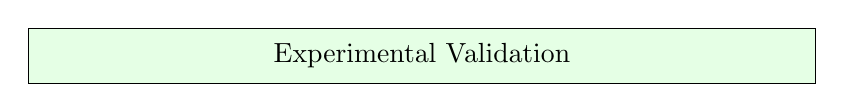
\begin{tikzpicture}
        \node[draw, rectangle, fill=green!10, minimum width=10cm, minimum height=0.7cm] {
            \begin{minipage}{9.5cm}
                \centering
               Experimental Validation 
            \end{minipage}
        };
    \end{tikzpicture}
    \end{center}
    \vspace{0.5cm}
    \centering
    \textbf{\textcolor{violet}{What is next ? }}
\end{frame}

\begin{frame}{Short-term perspectives}
    \begin{columns}[T]
        \begin{column}{0.33\textwidth}
            \centering
            \textbf{\textcolor{blue}{Optimal Torque Control}}

            \vspace{0.3cm}
            \small
            \begin{itemize}
                \item Extend the convex formulation to other types of machines
                \item Generic embedded solver for all synchronous machines
            \end{itemize}
        \end{column}

        \begin{column}{0.33\textwidth}
            \centering
            \textbf{\textcolor{blue}{Embedded Synthesis}}

            \vspace{0.3cm}
            \small
            \begin{itemize}
                \item Exploit the sparsity of the matrices
                \item Better tuning of the interior-point method (ADMM...)
                %\item
               % \item Guaranteed transient specifications
            \end{itemize}
        \end{column}

        \begin{column}{0.33\textwidth}
            \centering
            \textbf{\textcolor{blue}{LPV Control}}

            \vspace{0.3cm}
            \small
            \begin{itemize}
                \item Explore other nonlinear types of control (Sum-of-Squares)
                \item Include input and state saturations in the LMI synthesis
            \end{itemize}
        \end{column}
    \end{columns}
\end{frame}


